\section{Evaluation}\label{sec:eval}

% \milind{Need to intro evaluation here: 
% 1. what research questions we're trying to answer
% 2. high level overview of what we're going to evaluate to answer those questions
% 3. what platforms we're using to do the evaluation
% }

%\raghav{how's this?}
We would like to know whether \system's vectorization strategy actually leads to significant speedups on realistic applications, as well as what properties of a program affect \system's ability to vectorize it.
To answer these questions, we evaluate \system on a number of real-world kernels that represent both regular and irregular computation.
We also evaluate \system on a set of randomly fuzzed irregular microbenchmarks that vary aspects like computation density and homogeneity to investigate the effects of these properties on vectorizability. %\raghav{Further explain what that means here? Or wait until the microbenchmarks section?}\milind{wait}
All our experiments are run on a 2020 Apple M1 MacBook with 16 GB of memory. %\raghav{I don't need to say stuff about the cores etc. since nothing's being multithreaded, right?}\milind{Yeah, I think that's fine.}

\subsection{Computational Kernels}
\begin{figure}
	\vspace{-4em}
    \begin{subfigure}{\linewidth}
        \includegraphics[width=1\textwidth]{figures/newAspectRatioGraphs/DataUnreplicatedENC+RUN.png}
        \vspace{-3.5em}
        \caption{Scalar vs. Vector comparison for unreplicated inputs}\label{fig:ml-kernels-unrepl}
    \end{subfigure}
    
    \vspace{-2.5em}
    
    \begin{subfigure}{\linewidth}
        \includegraphics[width=1\textwidth]{figures/newAspectRatioGraphs/DataPartiallyReplicatedENC+RUN.png}
                \vspace{-3em}
        \caption{Scalar vs. Vector comparison for partially replicated inputs}\label{fig:ml-kernels-part-repl}
    \end{subfigure}
    
     \vspace{-3em}
     
    \begin{subfigure}{\linewidth}
        \includegraphics[width=1\textwidth]{figures/newAspectRatioGraphs/DataReplicatedENC+RUN.png}
            \vspace{-3.5em}
        \caption{Scalar vs. Vector comparison for fully replicated inputs}\label{fig:ml-kernels-repl}
    \end{subfigure}
    \caption{Scalar vs. Vector encryption + run time comparisons for various replication regimes. Scalar times (red) are normalized to 1, and a smaller (blue) vector bar is better.}\label{fig:ml-kernels}
\end{figure}

We evaluate \system by compiling several computational kernels, of the sort that might be found in machine-learning code, and comparing their vectorized performance against an unvectorized (scalar) baseline implementation. Both the scalar and vector versions use the same FHE backend.
Each of the matrix or vector inputs to the kernels are grouped into their own vectors as described in Section~\ref{sec:duplicating-inputs}.
%Although this can lead to worse schedules than if we didn't force groupings, we expect this to be the most common use case. \raghav{Is that what I wanna say? Or should I just combine it with the previous sentence and say ``yeah we force packings, yeah we know its not optimal.''}

Each kernel is used in two benchmarks with differently sized inputs and three different replication strategies: once with both inputs replicated, once with only one input replicated, and once with neither input duplicated. 
The exact benchmarks used are:
\begin{itemize}
    \item Matrix/Matrix multiply ($2 \times 2$ and $3 \times 3$)
    \item Matrix/Matrix multiply followed by determinant ($2 \times 2$ and $3 \times 3$)
    \item Pairwise distance computation (2 points and 3 points)
    \item Vector dot product (vector size of 3 and 6)
    \item Matrix convolution ($4 \times 4$ matrix with $2 \times 2$ kernel and $3 \times 3$ kernel)
\end{itemize}

Figure~\ref{fig:ml-kernels} shows the performance results for these benchmarks.
The red bars show the scalar execution time (normalized to 1), and the blue bars, the relative vector execution time (a smaller blue bar is better).
Vector execution ranges from 0.77 to 6.2 times faster than scalar execution.
Almost all benchmarks are substantially faster with vectorization, except those with lots of dependences (such as pairwise distance) or lots of reuse (such as matrix convolution), both of which result in a lot of data shuffling.

% \milind{Start with the punchline -- don't keep people in suspense: vector execution ranges from $0.xxx$ to $y$ times faster than scalar execution. Almost all benchmarks, except those with ... have substantially faster vector than scalar runtimes, and performing full replication, which means less rotation is needed, is uniformly faster -- up to 5 times faster. Once you give them the punchline, then you can explain the rest of the details.}

% Most of our benchmarks see a greater speedup from vectorization as we move from unreplicated inputs to fully replicated inputs.
% This is what we expect, because, as discussed in Section~\ref{sec:duplicating-inputs}, replicating a set of inputs leads to fewer rotations necessary to get each of them to the correct lanes.
Performing full replication ameliorates these problems (Section~\ref{sec:duplicating-inputs}), and is uniformly faster.
Fully-replicated vector benchmarks range from a 6.2$\times$ speedup for \texttt{mat\_mul2x2}, to an approximately $25\%$ speedup for \texttt{mat\-\_mul\-\_det3x3}

In the unreplicated runs, we see some of the vectorized kernels (\texttt{mat\-\_convol\-\_4x4x2x2}, \texttt{mat\-\_mul\-\_det3x3}, and \texttt{pair\-wise\-\_dist2x2}) are actually {\em slower} than the scalar baseline.
This is because the overhead of all the rotations these benchmarks incur outweighs any benefits gained from vectorization.
In fact, it makes sense that these benchmarks would behave like that: convolution is a computation with substantial data reuse, leading to a high number of rotations to move data.
The $2 \times 2$ pairwise distance benchmark has a fully-connected dependence graph, leading to essentially the worst case scenario for vectorization.
And computing the determinant at the end of \texttt{mat\_mul\_det3x3} requires a reduction of 9 values, with no symmetries between them to exploit.
However, even in these examples, the vectorized code is no more than 20\% worse than scalar, showing that despite the high rotation costs, \system is still able to properly take advantage of vectorization opportunities.
%\raghav{This all kind of seems like a jumble but I hope I'm getting the point across}

Overall, we see that it is almost always better to fully replicate inputs when vectorizing, unless specifically compiling several composable kernels separately. While it may seem that replicating data could increase overheads (e.g., by requiring more time to encrypt the input, or by requiring larger vector widths), in practice it does not. Encryption is vectorized in the same way as computation so does not take appreciably longer if the same data is encrypted multiple times. And vector widths in FHE are very high to begin with, so there is ample lane space to house the replicated data.

Visually inspecting the vector code generated by \system reveals that it often automatically finds what known optimal schedules.
For example, in the dot product kernels, \system first packs all of the multiplications into a single vector operation, then vectorizes the levels of the logarithmic reduction tree.\footnote{Note that the logarithmic reduction tree arises because the eDSL implementation of dot product uses a recursive sum operation---\system does not introduce new parallelism. Nevertheless, \system correctly exploits the parallelism that {\em does} exist in the circuit.}
In the \texttt{mat\_mul\_det} kernels, \system first identifies the the highly vectorizable matrix multiply part of the computation, vectorizes that, and then essentially computes the highly irregular determinant on a single lane.

% \milind{Add a discussion here about visually inspecting the generated code, and point out where and whether coyote does especially cool stuff, or where it breaks down.}

\subsubsection*{Ideal Speedups}

\begin{table}
\small
    \caption{Speedups from vectorization (ideal speedup by instruction count, and observed speedup by execution time)}\label{tab:ideal-speedup}
    \begin{tabular}{lcccc}
        \toprule    
        Benchmark & Ideal Speedup & Observed Speedup\\\midrule
        \texttt{mat\_convol\_4x4x2x2} & 3.225 & 1.560\\
        \texttt{mat\_mul\_det2x2} & 4.565 & 3.249\\
        \texttt{mat\_mul3x3} & 4.881 & 4.182\\
        \texttt{pairwise\_dist3x3} & 1.969 & 2.137\\
        \texttt{dot\_product3x3} & 2.667 & 1.999\\
        \texttt{pairwise\_dist2x2} & 1.292 & 1.279\\
        \texttt{dot\_product6x6} & 5.000 & 3.558\\
        \texttt{mat\_convol4x4x3x3} & 4.404 & 2.346\\
        \texttt{mat\_mul2x2} & 7.636 & 6.184\\
        \texttt{mat\_mul\_det3x3} & 1.799 & 1.153\\\bottomrule
    \end{tabular}
\end{table}

In addition to collecting data about execution time, we also model the ideal speedup of each benchmark (i.e., how much faster vectorization would be if data shuffling were free).
We do this by counting the instructions in both the fully replicated vector schedule and the baseline scalar code, treating a ciphertext multiply as being roughly 10$\times$ as expensive\footnote{This is also the ratio \system uses in its internal cost model.} as a ciphertext add or plaintext multiply, and treating each rotation as a no-op.
This data is shown in Table~\ref{tab:ideal-speedup}.
The most vectorizable benchmarks are \texttt{mat\_mul2x2} and \texttt{dot\_product6x6}, with ideal speedups of 7.6 and 5.0 respectively, and the least vectorizable benchmark is \texttt{pairwise\_dist2x2}, with an ideal speedup of approximately 1.3.
This is as expected: the first two are very regular computations, and the pairwise distance benchmark represents a worst case scenario for vectorization, due to its dense dependence structure.
However, all of these ideal speedups are close to the actual speedup in execution time as shown in the table, suggesting that \system is capable of finding highly optimized schedules even in the presence of high data movement costs. (Note that for \texttt{pairwise\_dist2x2}, the observed speedup is actually {\em higher} than the ideal speedup; this discrepancy is because the cost model used to calculate ideal speedups is an approximation.)
%\milind{Remove the scalar and vector columns from the table, and add an ``observed speedup'' column to the table so people can see that we get pretty close to the ideal speedup}

\paragraph{Compilation time}
Table~\ref{tab:compilationtime} shows the compilation time for each of the benchmarks. We see that the slowest compilation times occur for the un-replicated variants. We see that some of the larger benchmarks with many lane assignment problems to solve can take several minutes to complete. However, when weighed against the generally high cost of FHE execution, this compilation time is reasonable, and is in the same ballpark as other FHE vectorizers~\cite{Porcupine}.

\begin{table}
\small
	\caption{Compilation time (s) for \system benchmarks}
	\label{tab:compilationtime}
	\vspace{-0.5em}
    \begin{tabular}{lccc}
        \toprule
        Benchmark & Unreplicated & Partial & Replicated\\\midrule
        \texttt{mat\_convol\_4x4x2x2} & 143.998 & 249.587 &199.653\\
        \texttt{mat\_mul\_det2x2} & 3.702 & 2.386 &2.356\\
        \texttt{mat\_mul3x3} &  104.779 & 66.661&107.803\\
        \texttt{pairwise\_dist3x3} & 132.660 & 158.475&194.264\\
        \texttt{dot\_product3x3} & 0.425 & 0.304&0.332\\
        \texttt{pairwise\_dist2x2} & 9.582 & 11.984&15.737\\
        \texttt{dot\_product6x6} & 1.131 & 1.158&1.370\\
        \texttt{mat\_convol4x4x3x3} & 453.378 & 144.412&206.653\\
        \texttt{mat\_mul2x2} & 3.702 & 1.739&1.837\\
        \texttt{mat\_mul\_det3x3} & 307.757 & 382.387&476.384\\
        \bottomrule
    \end{tabular}
\end{table}


\subsection{Fuzzed Microbenchmarks}
To investigate how various aspects of program structure affect \system's ability to vectorize, we randomly generate several expression trees according to three regimes:
\begin{enumerate}
    \item {\em Sparse}: Many operations have one leaf node input, the tree is not very balanced
    \item {\em Dense, homogeneous}: The expression tree is both full and complete, and all the operations are isomorphic
    \item {\em Dense, nonhomogeneous}: The expression tree is both full and complete, each operation has a 50/50 chance of being an add or a multiply.
\end{enumerate}
We generate ten trees for each regime: five with a maximum depth of 3, and five with a maximum depth of 6.
The relative speedups for these trees are shown in Figure~\ref{fig:fuzzed-trees}.
We see that aside from the sparse trees of depth 3, all the rest show speedups when vectorizing, which makes sense since the sparse computations tend to be much more linear and have fewer opportunities for vectorization.
The depth 3 trees show on average less speedup than the depth 6 trees, since they also have less work available to vectorize, and less parallelism in their circuits. %\raghav{Is this true? I'm basically trying to say that the scalar is already not bad for a tiny tree so what's the point in vectorizing it}\milind{It's basically about less parallelism. For a complete tree, parallelism is n/log(n), so as n gets bigger, there is more parallelism --- a depth 6 tree has 4 times as much parallelism as a depth 3 tree}

\begin{figure}
    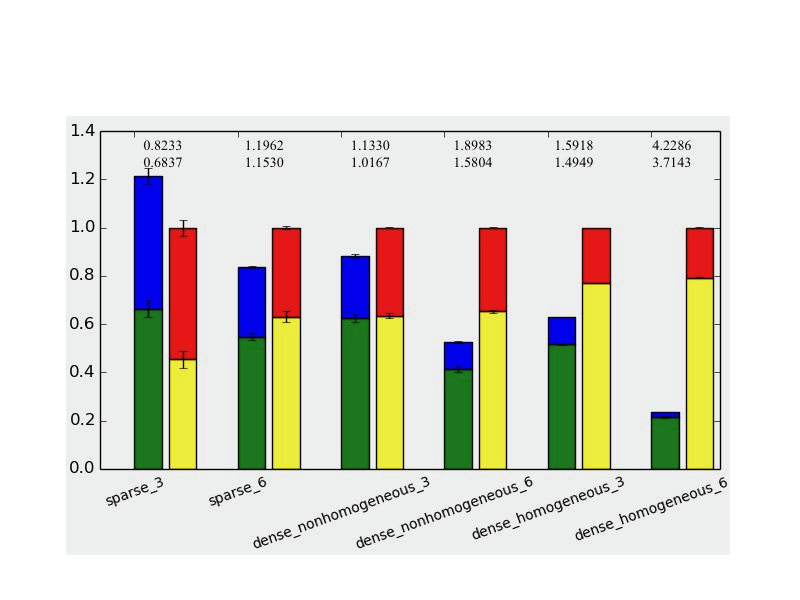
\includegraphics[width=0.9\columnwidth]{figures/graphs/TreeGraphwithNumbers.png}
    \vspace{-0.5em}
    \caption{Vectorization speedups on microbenchmarks. Blue/green bars represent vector time, and red/yellow bars represent (normalized) scalar time, with a smaller blue/green bar being better. Bars are split between time execution time and encryption time, with execution time on the bottom (green and yellow) and encryption time on top (blue and red). The numbers on top of the bars represent the speedup of vector over scalar, with the first one including encryption time and the second one excluding it.}\label{fig:fuzzed-trees}
\end{figure}